%%%%%%%%%%%%%%%%%%%%%%%%%%%%%%%%%%%%%%%%%
% University/School Laboratory Report
% LaTeX Template
% Version 3.1 (25/3/14)
%
% This template has been downloaded from:
% http://www.LaTeXTemplates.com
%
% Original author:
% Linux and Unix Users Group at Virginia Tech Wiki 
% (https://vtluug.org/wiki/Example_LaTeX_chem_lab_report)
%
% License:
% CC BY-NC-SA 3.0 (http://creativecommons.org/licenses/by-nc-sa/3.0/)
%
%%%%%%%%%%%%%%%%%%%%%%%%%%%%%%%%%%%%%%%%%

%----------------------------------------------------------------------------------------
%	PACKAGES AND DOCUMENT CONFIGURATIONS
%----------------------------------------------------------------------------------------

\documentclass[12pt]{article}
%\documentclass[14pt]{extarticle}

\usepackage{setspace} % For set space
\usepackage{algorithm} % For pseudo code
\usepackage[noend]{algpseudocode}
\usepackage{siunitx} % Provides the \SI{}{} and \si{} command for typesetting SI units
\usepackage{graphicx} % Required for the inclusion of images
\usepackage{amsmath} % Required for some math elements 
\usepackage{cite} % For citation
\usepackage{algpseudocode}  

\setlength\parindent{0pt} % Removes all indentation from paragraphs
\setlength{\parskip}{0.5em}

\renewcommand{\labelenumi}{\alph{enumi}.} % Make numbering in the enumerate environment by letter rather than number (e.g. section 6)
\renewcommand{\baselinestretch}{1.2}
%\usepackage{times} % Uncomment to use the Times New Roman font

%----------------------------------------------------------------------------------------
%	DOCUMENT INFORMATION
%----------------------------------------------------------------------------------------

\title{\large Multiple AI Competition in Self Developed Game \\ Term 2 Report \\ ESTR4998/4999} % Title

\date{\today} % Date for the report

\begin{document}


\maketitle % Insert the title, author and date

\begin{center}
\begin{tabular}{l r}
Partners: & XIAO Tianyi \\ % Partner names
& LUO Lu \\
Instructor: & Prof. Andrej Bogdanov % Instructor/supervisor
\end{tabular}
\end{center}
\newpage


%----------------------------------------------------------------------------------------
%	SECTION 1
%----------------------------------------------------------------------------------------

\begin{abstract}
	(some abstract)
\end{abstract}
 
%----------------------------------------------------------------------------------------
%	SECTION 2
%---------------------------------------------------------------------------------------
\section{Background}

\subsection{Previous Progress}
In the last semester, we have implemented the preliminary version of the game environment and $Q$-Learning agent. In this section, we will briefly reiterate our previous progress before introducing new progress and our opinions.
\subsubsection{Environment}
When we started to draft our proposal, original considerations for designing our environment included complexity, scalability and implemental difficulty. We hoped to design an environment which is easy to implement, complex enough to distinguish the power of different algorithms and can be reused for different game modes, including 1 player, 1 versus 1, and multi-players against multi-players.

Therefore, we designed a game similar to football, and the graph user interface for 1 versus 1 version can be found in figure 1. In this environment, each agent controls one player which is represented as a blue(team 0) or an orange(team 1) rounded rectangle. And the purpose of players is to shoot the ball, which is represented as a white ball, to goal of opponent team, which is represent as white rectangle in the left border(for team 0) and right border(for team 1).

The environment can output a list to represent the game state. For 1 versus 1 mode, the list will contain the position of the current player, the position of the opponent player and the position of the ball.

The environment can receive a list with size equal 2 from a player as input, the first element represents the direction and the second element represents the action, shoot or not. 

After receiving an action, we can call the reward function to calculate the reward of the given action, and return the reward as a scalar number to that agent.

\subsubsection{Agent}

In the last semester, we have finished the design of Q-Learning agent by following the algorithm provided in the background theory section. Moreover, our conclusion of the last term is that our game is too complicated to be trained by Q-Learning even for 1 vs 1 mode, even if we simplified input states.

The reason to simplify states is that the number of raw game states is an enormous figure even without considering the action space. The simplify function will replace the positions of opponent player and ball by logarithms of relative positions(distances) with base 10, which will compress the range of these 4 parameters from several hundred to 7. This will significantly reduce the size of Q-Table and make some simpler situations trainable, and we will discuss this later.


%----------------------------------------------------------------------------------------
%	SECTION 3
%----------------------------------------------------------------------------------------

\section{Implementation}

\subsection{Single Player Mode}
In the beginning stage of our project in this term, we found that it's hard to train AI to play our game with DQN. So to simplify the issue and solve our prolem better, we first implement a single player mode. Then with the experience from single player mode, we are finally able to train DQN AI that could play 1v1 mode with logic.\\\\
In this mode, we randomize the initialization of our player and ball. They will be put on the soccer field randomly when each episode begins.
\begin{figure}[H]
	\begin{center}
		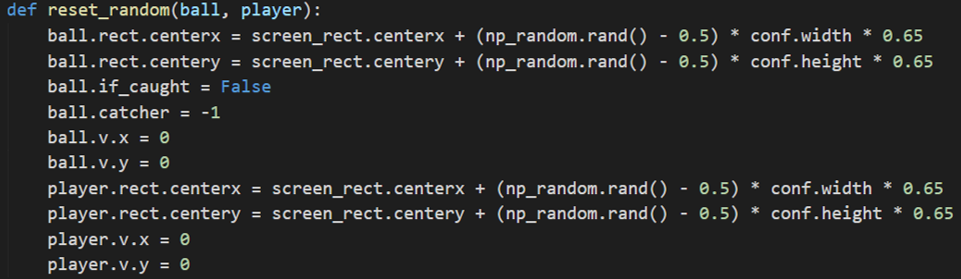
\includegraphics[width=0.9\textwidth]{reset_random}
		\caption{implementation of reset\_random}
	\end{center}
\end{figure}


\subsection{Agent State}
The state of agent represent the features sent to neural network. We add one more item into the agent state, which shows if the player is catching the ball or not. In the soccer game, there is cool down time for each player to prevent it to get the ball back as soon as it just shoots the ball. Therefore the coincidence of positions of player and ball doesn't mean that player could catch and shoot the ball. So one more item in agent state could help AI better understand its situation.\\\\


\subsection{Reward Function}
Reward function is crucial in reinforcement learning. As a soccer game, when a team get a goal, it will get huge reward. Besides, when a player catch a ball, it will also recive reward. Besides, to encourage player to keep the ball longer, once the player shoot the ball, it will get punishment.\\
However, only these basic rewards are not enough for training. Below are our modification for other part of reward function.

\subsubsection{Original Reward Function}
 In our original reward function, we give reward to the agent if it's closer to the ball than other player. Otherwise, the agent would get punishment. Besides, if the ball get closer to one door, the team attacking this door would get reward, and other team would get punishment.

\begin{algorithm}[!h]
	\caption{Original Reward$(Agent1,Agent2,Ball)$}
	\begin{algorithmic}
		\State Closer\_Agent(Agent1, Agent2, Ball).reward $+=$ 200
		\State Further\_Agent(Agent1, Agent2, Ball).reward $-=$ 200
		\If {Ball Moves right}
		\State Agent1.reward $+=$ 600
		\State Agent2.reward $-=$ 600
		\EndIf
		\If {Ball Moves left}
		\State Agent2.reward $+=$ 600
		\State Agent1.reward $-=$ 600
		\EndIf
		\If {Ball goes into right door}
		\State Agent1.reward $+=$ 100000
		\State Agent2.reward $-=$ 10000
		\EndIf
		\If {Ball goes into left door}
		\State Agent2.reward $+=$ 100000
		\State Agent1.reward $-=$ 10000
		\EndIf
		\If {Agent shoot the ball}
		\State Agent-shoot-ball.reward $-=$ 1000
		\EndIf
	\end{algorithmic}
\end{algorithm}

\subsubsection{Reward Function For Single Mode}
With Single Player Mode, we need a new reward function. This one is simple. If the player is moving closer to the ball, it will get reward, otherwise it will get punishment. Also, if the player shoot the ball to the direction to the right door, it will get reward. But if it shoots to wrong direction, it will get punishment. Then to encourage the player to keep the ball, it will also have reward when it keeps the ball.

\begin{algorithm}[!h]
	\caption{Single Mode Reward$(Agent,Ball)$}
	\begin{algorithmic}
		\If {Closer(Agent, Ball) or Keep(Agent, Ball)}
		\State Agent.reward $+=$ 200
		\Else
		\State Agent.reward $-=$ 200
		\EndIf
		\If {Ball goes into right door}
		\State Agent.reward $+=$ 100000
		\EndIf
		\If {Ball goes into left door}
		\State Agent.reward $-=$ 10000
		\EndIf
		\If {Agent shoot the ball}
		\State team-of-the-agent.reward $-=$ 1000
		\EndIf
	\end{algorithmic}
\end{algorithm}

\subsubsection{New Reward Function}
Then, with experience from single player mode, we modify our original reward function. We cancel the comparison of distance to ball between two agents, instead we only care if the agent is closer to the ball. Also, we cancel some punishment to avoid agent playing to negatively. And we adjust the amount of reward during our test.
\begin{algorithm}[!h]
	\caption{Original Reward$(Agent1,Agent2,Ball)$}
	\begin{algorithmic}
		\If {Closer(Agent1, Ball)}
		\State Agent1.reward $+=$ 100
		\Else
		\State Agent1.reward $-=$ 100
		\EndIf
		\If {Closer(Agent2, Ball)}
		\State Agent2.reward $+=$ 100
		\Else
		\State Agent2.reward $-=$ 100
		\EndIf
		\If {Ball Moves right}
		\State Agent1.reward $+=$ 100
		\EndIf
		\If {Ball Moves left}
		\State Agent2.reward $+=$ 100
		\EndIf
		\If {Ball goes into right door}
		\State Agent1.reward $+=$ 100000
		\State Agent2.reward $-=$ 10000
		\EndIf
		\If {Ball goes into left door}
		\State Agent2.reward $+=$ 100000
		\State Agent1.reward $-=$ 10000
		\EndIf
		\If {Agent shoot the ball}
		\State Agent-shoot-ball.reward $-=$ 1000
		\EndIf
	\end{algorithmic}
\end{algorithm}

\subsection{Neural Network}

\subsection{Measurement of Performance}


%----------------------------------------------------------------------------------------
%	SECTION 4
%----------------------------------------------------------------------------------------

\section{Result}

\subsection{Single Player Mode}

\subsection{1v1 Mode}


%----------------------------------------------------------------------------------------
%	SECTION 5
%----------------------------------------------------------------------------------------

\section{Discussion}



%----------------------------------------------------------------------------------------
%	BIBLIOGRAPHY
%----------------------------------------------------------------------------------------

\begin{thebibliography}{99}
	\bibitem{ref1}Silver, David, et al. "Mastering the game of Go with deep neural networks and tree search." nature 529.7587 (2016): 484-489.
	\bibitem{ref2}Mnih, Volodymyr, et al. "Playing atari with deep reinforcement learning." arXiv preprint arXiv:1312.5602 (2013).
	\bibitem{ref3}Berner, Christopher, et al. "Dota 2 with large scale deep reinforcement learning." arXiv preprint arXiv:1912.06680 (2019).
    \bibitem{ref4}Zoph, Barret, and Quoc V. Le. "Neural architecture search with reinforcement learning." arXiv preprint arXiv:1611.01578 (2016).
    \bibitem{ref5}Mnih, Volodymyr, et al. "Human-level control through deep reinforcement learning." nature 518.7540 (2015): 529-533.
\end{thebibliography}
%----------------------------------------------------------------------------------------


\end{document}